% Copyright 2021 Thomas Ascher
% SPDX-License-Identifier: CC-BY-SA-4.0

\documentclass[a4paper,parskip=half]{scrartcl}

\usepackage[T1]{fontenc}
\usepackage[ngerman]{babel}
\usepackage{csquotes}
\usepackage[regular,condensed,sfdefault]{roboto}
\usepackage{booktabs}
\usepackage{graphicx}
\usepackage{chemformula}
\usepackage{amsmath,amsfonts,amssymb}
\usepackage{icomma}
\usepackage{textcomp}
\usepackage{gensymb}
\usepackage[italic,symbolgreek]{mathastext}
\usepackage{float}
\usepackage[style=apa,backend=biber]{biblatex}
\DeclareLanguageMapping{ngerman}{ngerman-apa}
\usepackage[hidelinks,pdfencoding=auto,
  pdfauthor={Thomas Ascher},
  pdfusetitle,
  pdfkeywords={Bier,Refraktometer,Alkoholmessung,Terrill,Novotný}]{hyperref}
\usepackage{microtype}

\addto\extrasngerman{
\def\figureautorefname{Abb.}
\def\tableautorefname{Tab.}
\def\equationautorefname{Gl.}
}

\addto\captionsngerman{
\renewcommand{\figurename}{Abb.}
\renewcommand{\tablename}{Tab.}
}

\title{Alkoholmessung mit dem Refraktometer}
\author{Thomas Ascher <thomas.ascher@gmx.at>}
\date{7. September 2021, \href{http://creativecommons.org/licenses/by-sa/4.0/}{CC BY-SA 4.0}}

\addbibresource{refraktometer.bib}

\newcommand{\bxi}{\mathit{R}_i}
\newcommand{\bxitext}{$\smash{\bxi}$}
\newcommand{\bxic}{\mathit{Rc}_i}
\newcommand{\bxictext}{$\smash{\bxic}$}
\newcommand{\bxf}{\mathit{R}_f}
\newcommand{\bxftext}{$\smash{\bxf}$}
\newcommand{\bxfc}{\mathit{Rc}_f}
\newcommand{\bxfctext}{$\smash{\bxfc}$}
\newcommand{\sg}{\mathit{SG}}
\newcommand{\sgtext}{$\smash{\sg}$}
\newcommand{\abv}{\mathit{ABV}}
\newcommand{\abvtext}{$\smash{\abv}$}
\newcommand{\abw}{\mathit{ABW}}
\newcommand{\abwtext}{$\smash{\abw}$}
\newcommand{\oex}{\mathit{OE}}
\newcommand{\oextext}{$\smash{\oex}$}
\newcommand{\aex}{\mathit{AE}}
\newcommand{\aextext}{$\smash{\aex}$}
\newcommand{\rex}{\mathit{RE}}
\newcommand{\rextext}{$\smash{\rex}$}
\newcommand{\wcf}{\mathit{WCF}}
\newcommand{\wcftext}{$\smash{\wcf}$}
\newcommand{\adf}{\mathit{ADF}}
\newcommand{\adftext}{$\smash{\adf}$}
\newcommand{\rdf}{\mathit{RDF}}
\newcommand{\rdftext}{$\smash{\rdf}$}

\begin{document}
\maketitle

\section*{Einleitung}

Mittlerweile stehen dem Heimbrauumfeld eine breite Auswahl von Instrumenten
mit verschiedenen Messprinzipien zur Verfügung, die es ermöglichen, den
Alkoholgehalt eines selbst gebrauten Biers abzuschätzen oder den
Gärverlauf zu beobachten. Das ist neben der klassischen Bierspindel
unter anderem das Handrefraktometer. Die Refraktometrie ist
kein Neuankömmling im Bereich der Bieranalyse. Versuche,
auf Basis dieses Messprinzips den Alkoholgehalt zu bestimmen, reichen bis
in das Jahr 1843 zurück \parencite[102]{Gamer1959}.

Auch wenn Refraktometer den Ruf besitzen, weniger genaue Messergebnisse
zu liefern als andere labortechnische Instrumente, liegen deren
Vorteile klar auf der Hand: kurze Messzeiten bei geringem Probevolumen
und überschaubarer Bedienungskomplexität. Im Gegensatz zu den bei der
Bierspindel üblichen 100 Millilitern pro Probe werden nur wenig
Milliliter benötigt, die sich dementsprechend auch schneller nach dem
Hopfenkochen auf Messtempertur abkühlen lassen. \parencites[171\psq]{Bettner1969}{Terrill2011}

Wie nun Messungen mit einem Refraktometer während des Brau- und
Gärprozesses durchzuführen sind und sich darauf basierend der
Alkoholgehalt als Näherungswert berechnen lässt, wird
Rahmen dieses Artikels erörtert.

\section*{Messprinzip und Gerätetypen}

Wenn Licht auf eine Grenzfläche zwischen unterschiedlich optisch
dichten Medien (verschiedene Brechungsindexe) trifft,
kommt es zur Lichtbrechung und Reflexion. Dieser physikalische Effekt
wird in einem Refraktometer als Brechungsindex quantifiziert.
Maßgeblich zur Messwertbestimmung ist der materialabhängige
kritische Einfallswinkel ab dem keine Brechung mehr stattfindet
sondern das Licht in seiner Gesamtheit reflektiert wird.
Der Brechungsindex \(\mathit{nD}\) ist als Verhältnis zwischen der
Geschwindigkeit von Licht im Vakuum und einem Medium definiert. Je höher
die optische Dichte ist, desto größer ist auch der Brechungsindex.
\parencites{AKRSSOGH2021}[43]{Bonham2001}[102\psq]{Gamer1959}

Refraktion ist temperaturabhängig. Messungen sind daher je nach
Anwendungsgebiet bei einer festgelegten Temperatur durchzuführen.
Das sind im Normalfall 20~°C. Selbst kostengünstige Handrefraktometer
besitzen deshalb einen Kompensationsmechanismus (Automatical Temperature
Compensation, ATC) in Form eines Bimetallsteifens. Dieser 
verschiebt je nach Temperatureinwirkung zur Korrektur selbstständig
die Messskala des Geräts. Hierbei ist zu beachten, dass diese Form der
ATC nur für den kalibrierten Probentyp des Geräts ausgelegt ist.
\parencites{Depalma2017}{Distillique2020}{Gossett2012}[50]{Terrill2013}

Der Brechungsindex ist mitunter keine geeignete Messgröße für alle
technischen Prozesse. Deshalb wird dieser je nach Anwendungsgebiet
und Probe auf die gewünschte Messgröße kalibriert. Zur Messung
der relativen Dichte von Saccharose/Wasser-Lösungen im Bereich der
Wein- und Saftherstellung ist diese zum Beispiel Grad Brix (°Bx), wobei
ein °Bx einem Gramm Saccharose auf 99 Gramm Wasser entspricht.
\parencites[43]{Bonham2001}[50]{Terrill2013} Die Umrechnung zwischen
Brechungsindex und Grad Brix ist durch die ICUMSA
Tabellen normiert.

In den Shops für Heimbraubedarf werden im wesentlichen Refraktometer in
zwei verschiedenen Bauformen angeboten: analoge Handgeräte
und kompakte digitale Tischgeräte wie das für die Weinherstellung
gedachte \href{https://milwaukeeinstruments.eu/milwaukee-ma885-digital-brix-oechsle-oe-and-kmw-babo-refractometer/}{Milwaukee MA885} (\autoref{fig:refactotype},
\autoref{table:refactospec}). Beide Bauformen setzten Prismen zur
Lichtbrechung ein. Handrefraktometer funktionieren
nach dem Durchlichtprinzip. Vereinfacht dargestellt scheint dabei Licht
von einer externen Quelle durch die Probe, wird über Prismen gebrochen
und durch weitere optische Komponenten und eine Skala bis hin zu einem
Okular geleitet. Unterschiedliche kritische Winkel erzeugen dabei eine
andere Teilung des Sichtfelds, anhand der der Messwert abgelesen werden
kann (\autoref{fig:refractoscale}). Im Unterschied dazu besitzen
digitale Refraktometer eine interne Lichtquelle und erfassen die
Messung über einen CCD-Sensor. Das Licht muss dabei für die Brechung die Probe
nicht durchqueren. \parencites{AKRSSOGH2021}[102\psq]{Gamer1959}[50]{Terrill2013}
 
\begin{figure}[h]
\centering
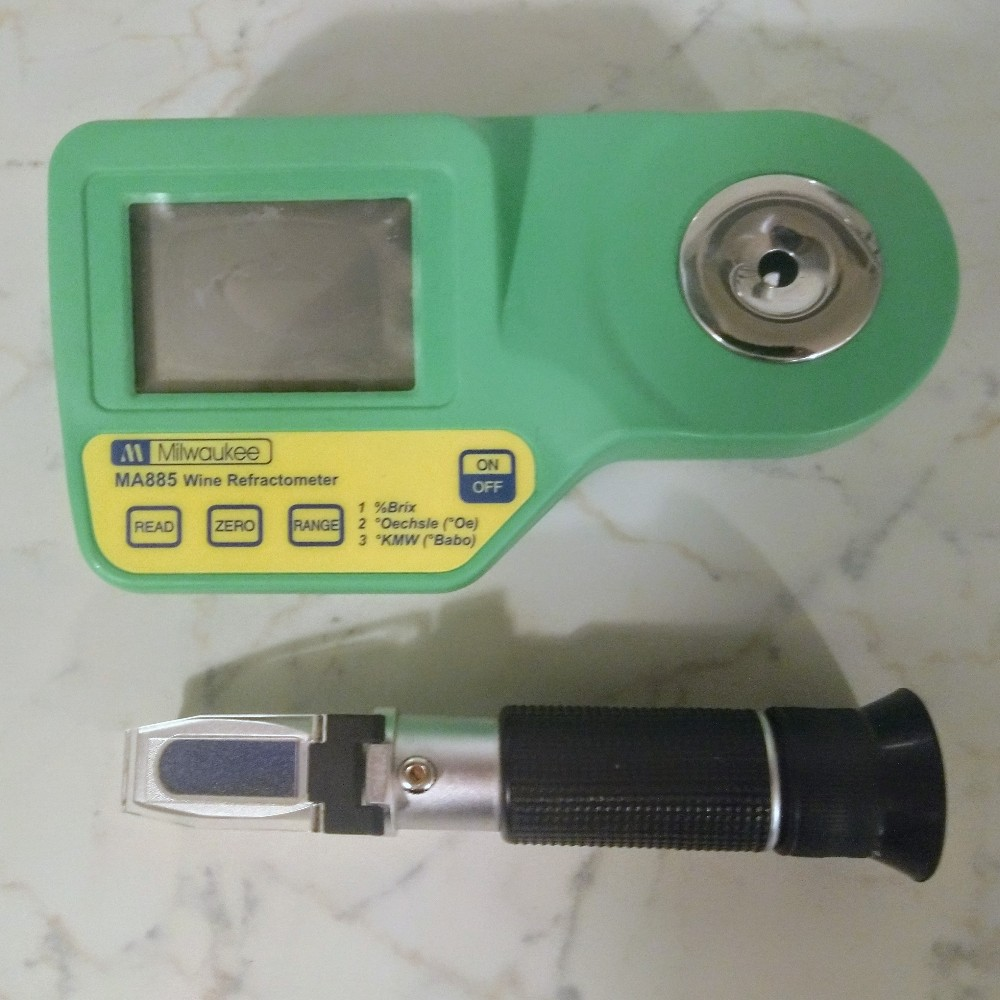
\includegraphics[width=4.8cm]{images/types.jpg}
\caption{Typische Refraktometer im Heimbraubereich (Ascher, 2021)}
\label{fig:refactotype}
\end{figure}

\begin{table}[h]
\centering
\begin{tabular}{lrr}
\toprule
Parameter &  Handrefraktometer &  Milwaukee MA885 \\
\midrule
Preis [€] & 40 & 185 \\
Messbereich [°Bx] & 0--32 & 0--50 \\
Auflösung [°Bx] & 0,2 & 0,1 \\
Genauigkeit [°Bx] & 0,2 & 0,1 \\
ATC [°C] & 10--30 & 10--40 \\
Maßeinheiten & °Bx, SG & °Bx, °Oe, °KWM \\
Kalibrierschein & nein & ja \\
\bottomrule
\end{tabular}
\caption{Spezifikation typischer Refraktometer im Heimbraubereich  (Ascher, 2021)}
\label{table:refactospec}
\end{table}

\begin{figure}[h]
\centering
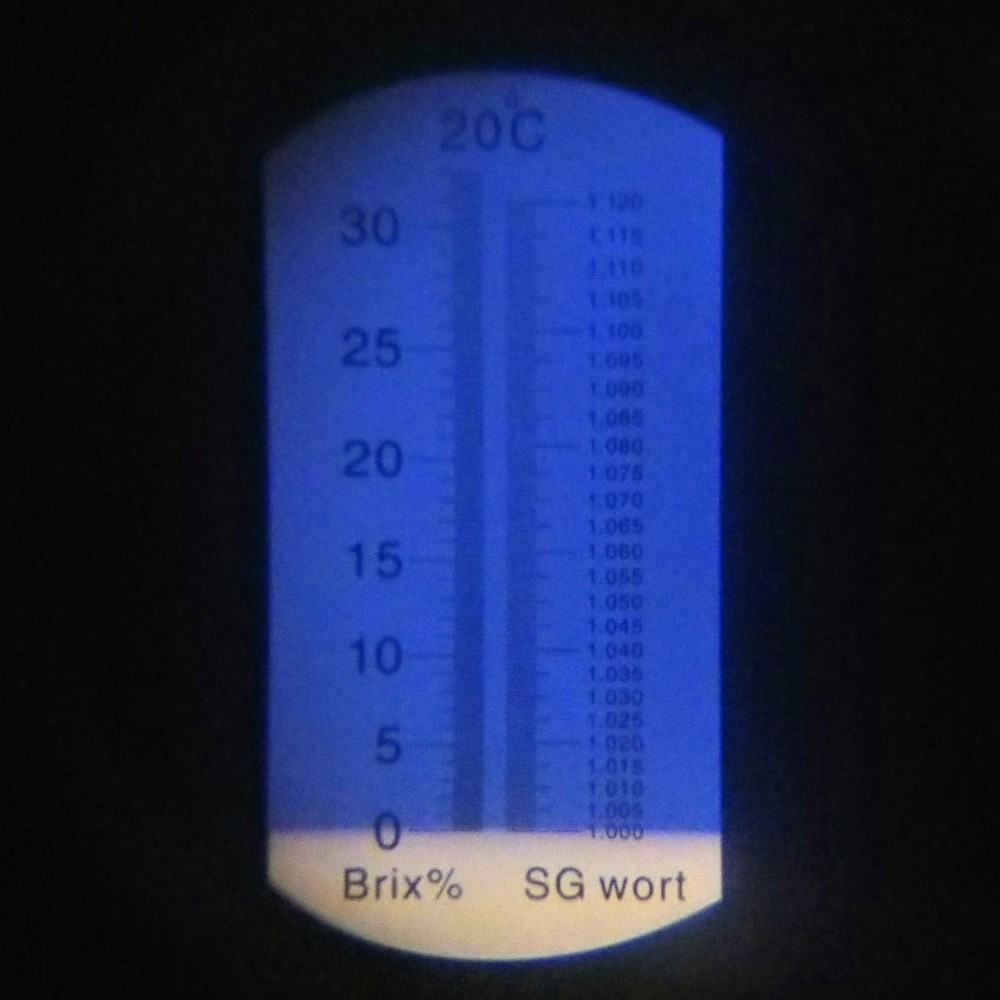
\includegraphics[width=4.8cm]{images/scale.jpg}
\caption{Durchsicht durch ein Handrefraktometer (Ascher, 2021)}
\label{fig:refractoscale}
\end{figure}

\section*{Exkurs Bierspindel}

Für Vergleichsmessungen zu einem Refraktometer oder zur Kalibrierung
des refraktometerspezifischen Würze-Korrekturfaktors (Wort Correction
Factor, \wcftext) wird in Heimbraubereich meist eine Bierspindel
eingesetzt. Darüber hinaus decken sich die Berechnungswege für
den Alkoholgehalt und weiterer Kennzahlen für beide Messgeräte, da
mit einem Refraktometer erfasste Messwerte üblicherweise in
Spindelwerte umgerechnet werden.

Eine Bierspindel (auch Saccharometer) ist ein auf Massenanteil
kalibriertes Aräometer. Mit einem Aräometer lässt die
spezifische Dichte (Specific Gravity, \sgtext) einer Flüssigkeit auf
Basis des Archimedischen Prinzips messen. Das heißt, dass ein in
Flüssigkeit eingetauchter Körper Auftrieb in dem Maß der Gewichtskraft
der dabei verdrängten Flüssigkeit erfährt. Je geringer die Dichte einer
Flüssigkeit dabei ist, desto weiter sinkt ein Körper ein. Hierbei ist zu
beachten, dass die Dichte temperaturabhängig ist. Daher wird für die
spezifische Dichte eine Referenztemperatur angegeben. Für die
in diesem Artikel beschriebenen Angaben und Berechnungen entspricht
diese 20~°C. Bei Abweichungen von dieser Referenz ist eine
Messwertkorrektur durchzuführen. Messwerte müssen von der Skala je nach
Aräometer über oder unter dem gebildeten Flüssigkeitsmeniskus abgelesen
werden.
\parencites[324\psqq]{Kunze2004}[647\psq]{Narziss2009}[131]{Spedding2016}

Für verschiedene Abschnitte im Brauprozess existieren spezialisierte
Spindelausführungen. Das sind die universelle, auf 20~°C kalibrierte
Sudhausspindel, die zum Läutern auf 70~°C kalibrierte Läuterspindel
mit weniger feiner Graduierung (rote Kennzeichnung) und die auf die
Gärung und Kellertemperaturen ausgelegte Keller-/Endvergärungsspindel (grüne
Kennzeichnung) \parencite[381\psqq]{Brueckelmeier2018}.

In den USA führen Heimbrauer:innen Spindelmessungen zumeist
mit einem Hydrometer durch um die relative Dichte von Würze in
Bezug auf Wasser festzustellen. Die Skala einer Bierspindel ist hingegen
auf Grad Plato kalibriert. Grad Plato (°P) ist das Maß für die vor der
Gärung gemessene Stammwürze eines Bieres (Original Extract, \oextext),
wobei ein °P einem Gramm Extrakt auf 100 Gramm Bier entspricht. Mit
Extrakt sind vor allem die Bestandteile gemeint, die während des
Maischeprozesses aus dem Malz gelöst werden. Die Umrechnung zwischen
Massenanteil in °P und der Massendichte
erfolgt auf Basis der Plato Tabellen über die Lincoln Gleichungen
(\autoref{eq:calcptosg}, \autoref{eq:calcsgtop}) oder vergleichbaren
Näherungsverfahren.
\parencites[648]{Kunze2004}[126,140\psq]{Spedding2016}

\begin{equation}
\sg\:[g/ml] = \frac{\degree P}{258,6 - \mathit{P} / 258,2 \cdot 227,1} + 1
\label{eq:calcptosg}
\end{equation}

\begin{equation}
\degree P\:[g/100g] = -205,347 \cdot \sg^2 + 668,72 \cdot \sg - 463,37
\label{eq:calcsgtop}
\end{equation}

Während und nach einer Gärung kann der scheinbare Restextrakt
(Apparent Extract, \aextext) gemessen werden. Scheinbar
deshalb, weil der während der Gärung gebildete Alkohol die
Dichte der Flüssigkeit verändert und somit den Messwert
verfälscht. Der wirkliche Restextrakt (Real Extract, \rextext)
entspricht nämlich einem höheren Betrag. Das ebenfalls
in Gärproben oder in Jungbieren enthaltene \ch{CO2} hat
ebenfalls einen Einfluss auf den Messwert. Es erhöht
diesen um circa 0,3~°P.
\parencites[53]{Novotny2017}[125]{Spedding2016}

Für genaue Messergebnisse sollten Spindeln mit einem möglichst
geringen Messbereich eingesetzt werden. In Heimbraushops sind
zum Beispiel Saccharometer mit einem Messbereich von 7~°P
und einer Graduierung von 0,1~°P erhältlich. Der geringe Messbereich
ermöglicht eine einfachere Ablesung und eine feinere Graduierung.
Für Hydrometer empfiehlt die Mitteleuropäische Brautechnische
Analysenkommission (MEBAK) Messgeräte die der DIN 12791-1 Norm
entsprechen. Darüber hinaus sollten folgende Vorgehensweisen
eingehalten werden \parencites[143]{MEBAK2013}[647\psq]{Narziss2009}{Wolf2015}:

\begin{itemize}
\item Eine Probe ist auf die ungefähre Temperatur des
Messgeräts abzukühlen oder zu erwärmen. Um eine Verdunstung
zu vermeiden ist die Probe abzudecken.
\item Proben sind vor der Messung gut zu durchmischen.
\item Während oder nach einer Gärung entnommene Proben sind
durch mehrmaliges Schütteln zu entgasen. Am Messgerät
anhaftende Gasblasen lassen sich sind durch schnelles eintauchen
in und herausziehen aus der zu messenden Probe entfernen.
\item Messgerät und Messgefäß sollten trocken und rein sein
und in der Waage stehen.
\item Das Messgefäß sollte die Bierspindel oder das Hydrometer
ohne großen Spielraum aufnehmen können.
\item Beim Ablesen des Messwerts ist die gegebenenfalls aufgedruckte
Leserichtung der Spindel zu berücksichtigen und danach die
Temperaturkorrektur auf 20~°C durchzuführen.
\end{itemize}

Im Jahr 2017 wurde ein Ringversuch zur Feststellung der „Gesamt­gü­te“
von Heimbrauer:innen eingesetzten Bierspindeln und Refraktometern im
Vergleich zu labortechnischen Geräten des Unternehmens Anton Paar anhand
zwei Referenzproben durchgeführt. Dabei hat sich gezeigt, dass mit
Präzisionsspindeln erhobene Messwerte nur geringe Abweichungen zu den
Ergebnissen des Laborgeräts aufweisen. Im Durchschnitt und im Extremfall
erzeugen kostengünstige Refraktometer jedoch geringere Abweichungen als
kostengünstige Bierspindeln. Dabei ist jedoch zu beachten, dass
die bei Refraktometern notwendige Umrechnung des Messwerts eine
zusätzliche Abweichung von bis zu 0,42~g/100g verursachen kann.
\parencite{Sauseng2017}

\section*{Messung}

Vor einer Messung sollte der Probenaufnahmebereich eines Refraktometers
und die zum Transfer der Probe eingesetzte Pipetten mit destilliertem Wasser
gereinigt werden, um eine Messwertverfälschung durch Rückstände vorheriger
Proben zu verhindern. Neben Kontaminierungen ist die Temperatureinwirkung
einer der häufigsten Quellen für Messfehler. Das eingesetzte Refraktometer
sollte daher auf Raumtemperatur erwärmt sein. Danach ist eine 
Einpunkt-Kalibrierung durchzuführen. \parencite{Depalma2017}

Proben bedürfen einer Aufbereitung. Darin enthaltene Schwebestoffe und
Gase sind zu entfernen. Das heißt, dass
während der Gärung entnommen Proben längere Zeit stehen gelassen werden
müssen, bis ein Großteil der darin enthaltenen Hefe sedimentiert
ist. Zur Entfernung von \ch{CO2} kann die Probe innerhalb eines
Behälters mehrmals geschüttelt werden. Inzwischen ist der Behälter
kurz zu öffnen, damit das Gas entweichen kann. Heiße Würze
sollte nicht direkt auf ein Refraktometer aufgetragen werden,
da es hierbei zu Verdampfungen kommt und somit zu einer
Konzentrationsänderung. Proben sind daher,
bis diese die Raumtemperatur angenommen haben, in einem abgedeckten
Behälter aufzubewahren. \parencites[105]{Gamer1959}[140\psq,150\psq]{MEBAK2013}[51\psq]{Terrill2013}

Für die eigentliche Messung sind mittels Pipette einige Tropfen
der Probe auf den Probenaufnahmebereich aufzutragen
(\autoref{fig:refactomeasure}). Beim Handrefraktometer
ist danach die Abdeckung zu schließen und dann das Messgerät
zum Ablesen des Messwerts gegen eine Lichtquelle zu richten.
Der Betrag des gemessenen Werts wird durch die Trennlinie zwischen
farblichem und farblosem Bereich signalisiert (\autoref{fig:refractoscale}).
Ist die Trennlinie verschwommen, befinden sich mitunter Schwebestoffe
in der Probe. Beim MA885 wird die Messung nach
dem Einschalten durch Drücken der Taste „Read“ ausgelöst. Der
Messwert ist danach vom Display abzulesen. Bei digitalen
Refraktometern ist zu beachten, dass durch externe Lichtquellen
verursachte Interferenzen die Messung beeinflussen können.
\parencites{Gossett2012a}[50\psqq]{Terrill2013}

\begin{figure}[h]
\centering
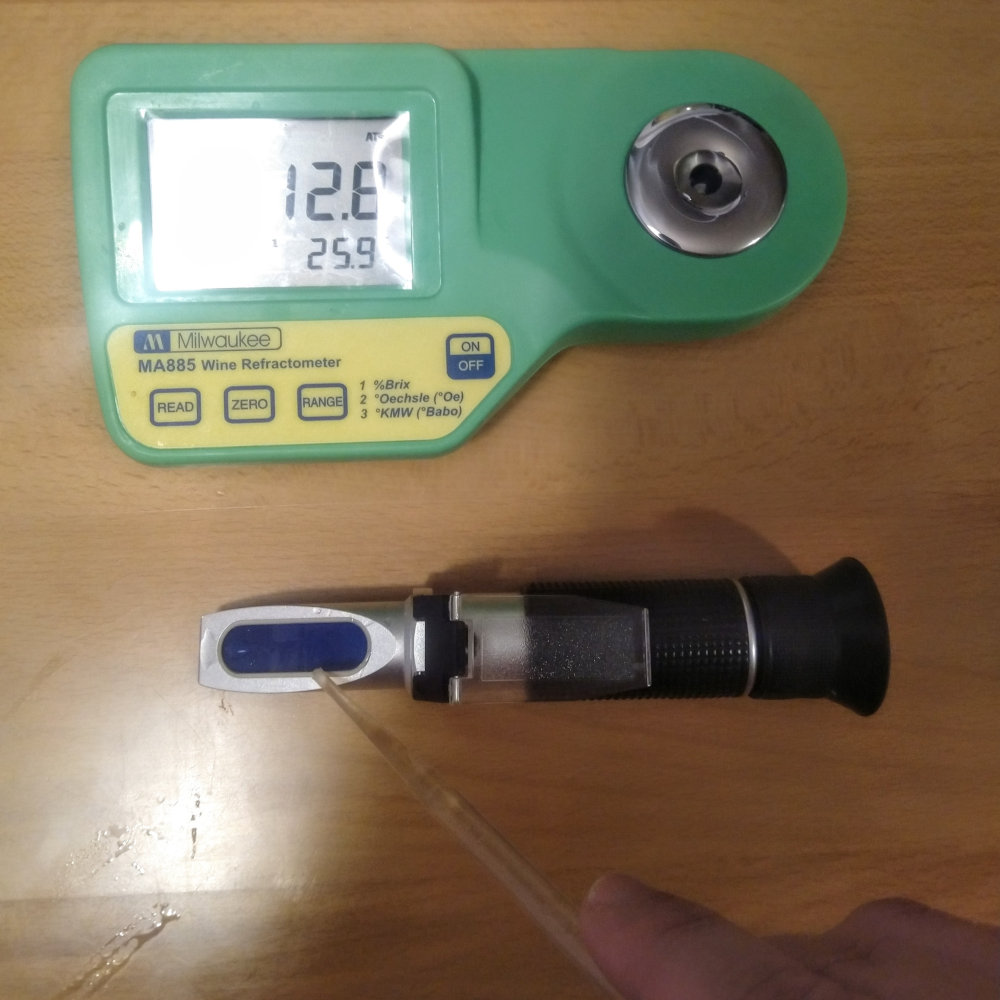
\includegraphics[width=4.8cm]{images/measure.jpg}
\caption{Durchführung einer Messung (Ascher, 2021)}
\label{fig:refactomeasure}
\end{figure}

\section*{Kalibrierung und Justierung}

Um sicherzustellen, dass ein Messgerät dauerhaft genaue Messergebnisse
liefert, ist in regelmäßigen Abständen eine Kalibrierung durchzuführen.
Das heißt, den mit dem Messgerät erfassten Messwert mit einer bekannten
Referenz (rückführbarer Kalibrierstandard) zu vergleichen und die
Abweichung festzustellen. Das sind bei Refraktometern zum Beispiel
wässrige Zuckerlösungen mit einem definierten Zuckergehalt.
Wird eine unerwünschte Abweichung festgestellt, kann diese
durch Justierung des betroffenen Messgeräts ausgeglichen werden.

Eine Kalibrierung ist je nach Anzahl der gemessenen Referenzen
eine Einpunkt-, Zweipunkt- oder Mehrpunkt-Kalibrierung.
Bei der Einpunkt-Kalibrierung wird im Wesentlichen ein definierter
Nullpunkt gesetzt. Die Erfassung von mehreren Messpunkten erlaubt
die Korrektur von linearen oder nicht linearen Abweichungen
über den Messbereich. Ab zwei Messpunkten kann eine Ausgleichsgerade
bestimmt und ab drei Messpunkten eine Polynomfunktion eingepasst
werden. \parencite{Earl2015}

Vor jeder Messserie empfiehlt sich die Durchführung einer
Einpunkt-Kalibrierung bei Raumtemperatur mit destilliertem
Wasser. Ein Refraktometer solle dabei die Raumtemperatur
angenommen haben und gereinigt sein. Zur Kalibrierung ist
eine Messung mit destilliertem Wasser als Probe durchzuführen.
Der abgelesene Messwert muss 0~°Bx betragen
(\autoref{fig:refractoscale}).
Wird eine Abweichung festgestellt, kann ein Handrefraktometer durch
Drehen an der Einstellschraube justiert werden (\autoref{fig:refactoadjust}),
bis die Anzeige 0~°Bx beträgt. Beim MA885 erfolgt die
Justierung durch Drücken der Taste „Zero“.
\parencites[44]{Bonham2001}{Depalma2017}[50\psq]{Terrill2013}

\begin{figure}[h]
\centering
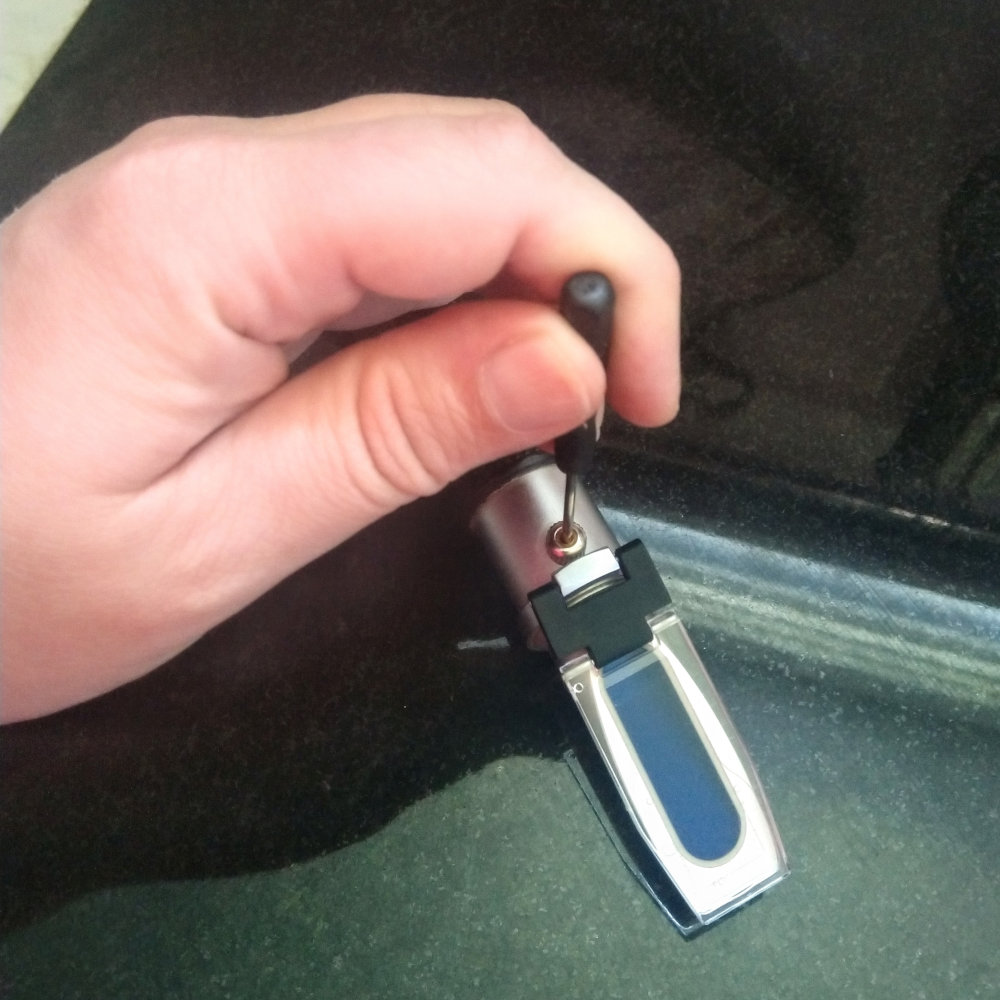
\includegraphics[width=4.8cm]{images/adjust.jpg}
\caption{Justierung eines Handrefraktometers (Ascher, 2021)}
\label{fig:refactoadjust}
\end{figure}

Messgeräte sollten nach der Herstellung einer ausreichenden
Qualitätssicherung unterlaufen. Bei günstigen Handrefraktometern
muss dies nicht zwangsweise der Fall sein \parencite{Troester2012}.
Zur Feststellung,
ob die integrierte Messskala eine zufriedenstellende Abdeckung
des Messbereichs bietet, lässt sich eine Zweipunkt-Kalibrierung
durchführen \parencites{Earl2015}[50\psq]{Terrill2013}. Da der Preis
eines Kalibrierstandards im Normalfall
deutlich über den Anschaffungskosten des Messgeräts
liegen, kann stattdessen eine Referenzlösung mit Haushaltszucker,
destilliertem Wasser und einer Feinwaage hergestellt werden. Zuerst
ist beim betroffenen Refraktometer, wie zuvor beschrieben, der
Nullpunkt zu kalibrieren und justieren. Danach ist eine Referenzlösung
für den oberen Bereich der Messskala herzustellen. Eine Lösung 
für 32~°Bx entspricht dabei 32~g Zucker auf 68~g Wasser.
Die festgestellte Abweichung lässt sich nicht justieren aber
durch Aufstellen einer Geradengleichung korrigieren.

\section*{Würze-Korrekturfaktor und Stammwürze}

Während sich die Einheit °Bx auf den Zuckeranteil in wässrigen Saccharoselösungen bezieht, beschreibt °P den Extraktgehalt. Ein
auf °Bx kalibriertes Refraktometer
sollte daher bei gleicher Stammwürze einen
höheren Messwert anzeigen als eine Bierspindel. Der Grund dafür ist,
dass Extrakt neben verschiedenen Zuckern noch weitere Bestandteile enthält, die
sich auf den Brechungsindex auswirken. Das sind unter anderem Säuren, Salze,
Proteine und Hopfenöle. Messwerte müssen dementsprechend durch einen
Korrekturfaktor (Wort Correction Factor, \wcftext) angepasst
werden. Zur Ermittlung der Stammwürze in °P ist daher 
der Messwert des Refraktometers der Stammwürze (\bxitext) gemäß
\autoref{eq:applywcf} durch den \wcftext\,zu dividieren.
\parencites[43]{Bonham2001}{BSHB2010}[119]{Roberts1950}[51]{Terrill2013}

\begin{equation}
\oex \:[\degree P] = \bxic = \frac{\bxi}{\wcf}
\label{eq:applywcf} 
\end{equation}

Der \wcftext\,ist stark von der Würzezusammensetzung und zum Teil
auch vom eingesetzten Messgerät abhängig und
sollte deshalb pro unterschiedlicher Schüttung mithilfe einer
Extraktmessung durch ein anderes Messgerät gemäß \autoref{eq:calcwcf}
bestimmt werden. Der etablierte Durchschnittswert für den
\wcftext\, entspricht 1,04 und bezieht sich auf die Messdifferenz
zu einem Pyknometer.
\parencites[44]{Bonham2001}[119]{Roberts1950}[51]{Terrill2013}

\begin{equation}
\wcf = \frac{\bxi}{\oex} \approx 1,04
\label{eq:calcwcf} 
\end{equation}

\section*{Korrelationsmodelle und scheinbarer Restextrakt}

Das während der Gärung gebildete Ethanol verfälscht nicht nur
die Extraktmessung mit der Bierspindel, sondern beeinflusst auch
den Brechungsindex. Es besteht daher die Notwendigkeit, einen
Refraktometermesswert für die Berechnung des Alkoholgehalts in eine
andere Messgröße zu transformieren. Die entsprechende Messgröße ist
im Normalfall der scheinbare Restextrakt, so wie er mit einer
Bierspindel gemessen würde. Die Umrechnung erfolgt durch eine
Korrelationsfunktion. Insgesamt wurden mindestens fünf
Korrelationsmodelle im Heimbrauumfeld für diesen Zweck veröffentlicht,
die ihre jeweiligen Stärken und Schwächen besitzen. Ein grundlegendes
Problem bei der Entwicklung eines solchen Modells ist,
dass verschiedene Zusammensetzungen einer vergorenen
Probe den gleichen Brechungsindex aufweisen können. \parencites{Distillique2020}{Terrill2010a}{Terrill2010}

Zur Berechnung der folgenden Korrellationsfunktionen ist eine
Probe der Anstellwürze vor der Gärung (\bxitext) und eine während
oder nach der Gärung entnommene Probe (\bxftext) mit einem Refraktometer
zu messen. Je nach Funktion sind unveränderte (\bxitext, \bxftext)
oder um den Würze-Korrekturfaktor angepasste Messwerte
(\bxictext, \bxfctext) einzusetzen.

\subsection*{Gardner}

Das lineare Gardner Modell zu Berechnung des scheinbaren Restextrakts
(\autoref{eq:gardner}) wurde im Jahr 2000 in der Zeitschrift
„The New Brewer“ veröffentlicht und von existierenden Gleichungen
abgeleitet. Bonham beschreibt dieses Modell als ausreichend
genau für die private Anwendung, weißt aber darauf hin, dass bereits
bessere Näherungsverfahren zu diesem Zeitpunkt existiert
hätten. Neben der Gleichung zur Bestimmung des scheinbaren
Restextrakts hat Gardner auch eine Gleichung zur Bestimmung
des Alkoholgehalts in Gewichtsprozent (Alcohol by Weight, \abwtext, \autoref{eq:gardnerabw}) aufgestellt. \parencite[44]{Bonham2001}
Im Heimbraubereich scheint dieses Modell keine große Verbreitung
erfahren zu haben.

\begin{equation}
\mathit{AE}\:[g/100g]=1,53 \cdot \bxf - 0,59 \cdot \bxic
\label{eq:gardner} 
\end{equation}

\begin{align}
\begin{split}
\abw\:[\%\:w/w] &= 1,09 \cdot \bxf - 1,13 \cdot \aex
\end{split} \label{eq:gardnerabw} 
\end{align}

\subsection*{Bonham}

Das von Bonham im Jahr 2001 im Zymurgy Magazin der American Homebrewers
Association veröffentlichte Korrelationsmodell ist auch als
Standardformel bekannt. Als Grundlage dienten bereits existierende
Gleichungen, die an die üblichen Messgrößen der amerikanischen
Heimbrauszene angepasst wurden. Bis zur Ablösung durch die Terrill
Formel ab dem Jahr 2011 war dieses Modell weit verbreitet. Heute
wird es noch vereinzelt wie zum Beispiel von 
„\href{https://www.maischemalzundmehr.de/index.php?inhaltmitte=toolsrefraktorechner}{Maische, Malz und Mehr}“ für Messungen während der Gärung empfohlen. \parencites[44]{Bonham2001}{Terrill2010a}

Das Bonham Modell besteht aus einer Gleichung zur Bestimmung der
spezifischen Dichte eines vergorenen Bieres (\autoref{eq:bonham})
und einer Gleichung zur Bestimmung des Alkoholgehalts in Volumenprozent
(Alcohol by Volume, \abvtext, \autoref{eq:bonhamabv}).

\begin{align}
\begin{split}
\sg\:[g/ml] &= 1,001843 - 0,002318474 \cdot \bxic - 0,000007775 \cdot \bxic^2 -
0,000000034 \cdot \bxic^3 \\
& \quad + 0,00574 \cdot \bxf +
0,00003344 \cdot \bxf^2 + 0,000000086 \cdot \bxf^3
\end{split} \label{eq:bonham} 
\end{align}

\begin{align}
\begin{split}
\abv\:[\%\:v/v] &= (277,8851 - 277,4 \cdot \sg + 0,9956 \cdot \bxf + 0,00523 \cdot \bxf^2 + 0,000015 \cdot \bxf^3) \\
& \quad \cdot \sg / 0,79
\end{split} \label{eq:bonhamabv} 
\end{align}

\subsection*{Terrill}

Bei Vergleichsmessungen zwischen einem Hydrometer und einem Handrefraktometer
in Verbindung mit der Bonham Gleichung hat Terrill im Jahr 2010 eine
mittlere Abweichungen der Messwerte von 1,3~g/100g festgestellt und darauf hin mit der Entwicklung eines eigenen Korrelationsmodell begonnen, welches
er in linearer (\autoref{eq:terrilllinear}) und vereinfachter kubischer Form
(\autoref{eq:terrillcubic}) veröffentlicht hat. \parencite{Terrill2010a}

\begin{equation}
\sg\:[g/ml] = 1 - 0,00085683 \cdot \bxic + 0,0034941 \cdot \bxfc
\label{eq:terrilllinear} 
\end{equation}

\begin{align}
\begin{split}
\sg\:[g/ml] &= 1 - 0,0044993 \cdot \bxic + 0,011774 \cdot \bxfc + 0,00027581 \cdot \bxic^2 - 0,0012717 \cdot \bxfc^2 \\
& \quad  - 0,0000072800 \cdot \bxic^3  + 0,000063293 \cdot \bxfc^3
\end{split} \label{eq:terrillcubic} 
\end{align}

Insgesamt dienten Vergleichsmessungen von 12 Bieren mit Stammwürzen
von 9 bis 24~°P, scheinbaren Restextrakten von 1,8 bis
5,6~g/100g und scheinbaren Vergärungsgraden von 73 bis 91~\%
als ursprüngliche Datenbasis. Messungen mit geringeren
Vergärungsgraden wurden ausgeschlossen, da diese die Genauigkeit des
Modells verschlechtert hätten.
\parencite{Terrill2010a,Terrill2011,Terrill2010}

\autoref{table:terrillcomp} zeigt den von Terrill veröffentlichten
Vergleich zwischen dem Modell von Bonham und seinem Eigenen. Bei
endvergorenen Proben erzeugt das Bonham Modell höhere
Abweichungen. Hierbei ist allerdings zu beachten, dass
Terrill die ursprüngliche Quelle des Bonham Modells nicht bekannt war
und deshalb fälschlicherweise auch den Messwert nach der Gärung um
den Würze-Korrekturfaktor angepasst hat. Dieser Fehler soll sich
aber nicht signifikant auf das Vergleichsergebnis auswirken.
\parencite{Terrill2010a,Terrill2011,Terrill2010}

\begin{table}[h]
\centering
\begin{tabular}{lrrr}
\toprule
Statistik & BO & TK & TL \\
\midrule
Max. Abw. [g/100g] & -2,1 & 1,2 & 1,0 \\
Mittlere Abw. [g/100g] & -0,4 & 0,2 & 0,0 \\
Standardabw. [g/100g] & 0,6 & 0,3 & 0,4 \\
Abw. < 0,25 g/100g [\%] & 18 & 56 & 63 \\
Abw. < 0,50 g/100g [\%] & 41 & 85 & 84 \\
Abw. < 1,00 g/100g [\%] & 90 & 97 & 99 \\
\bottomrule
\end{tabular}  \\
\vspace{2mm}
\small{BO=Bonham, TK=Terrill Kub., TL=Terrill Lin.}
\caption{Vergleich zwischen Bonham und Terrill Modell \parencite{Terrill2011}}
\label{table:terrillcomp}
\end{table}

\subsection*{Gossett}

Von den zuvor beschriebenen Korrelationsmodellen wird ein indirekter
Messwert in einen anderen transformiert. Gossett
war unzufrieden mit diesem Vorgehen und hat im Jahr 2012 daher ein
stöchiometrisches Modell (\autoref{eq:gossett}, \autoref{eq:gossettabw})
entwickelt, welches direkt den Alkohol in Gewichtsprozent auf Basis
von Refraktometermesswerten berechnet. Er hat hierzu die Auswirkungen
der Ethanolkonzentration
auf die Messwerten eines Refraktometers analysiert. Ein Gewichtsprozent
verfälscht diesen bei 20~°C um 0,445~°Bx. 
\parencite{Gossett2012,Gossett2012a,Gossett2012b}

\begin{equation}
C = 100 \cdot \frac{\bxi - \bxf}{100 - 48,4 \cdot 0,445 - 0,582 \cdot \bxf}
\label{eq:gossett} 
\end{equation}

\begin{equation}
\abw\:[\%\:w/w] = \frac{48,4 \cdot C}{100 - 0,582 \cdot C}
\label{eq:gossettabw} 
\end{equation}

Mit dem Gossett Modell lässt sich direkt keine spezifische Dichte
zur Berechnung von \autoref{eq:calcabv} bestimmen. Gossett wendet
hierzu \autoref{eq:bonham} an. Durch Umformung von
\autoref{eq:calcre} und \autoref{eq:calcabw} ist aber eine Berechnung
aus dem durch \autoref{eq:gossettabw} erhaltenen Alkoholgehalt möglich.

\begin{equation}
\aex\:[g/100g] = \bxi - \frac{\abw \cdot (2,0665 - 1,0665 \cdot \bxi / 100)}{0,8052}
\label{eq:gossettcor}
\end{equation}

\subsection*{Novotný}

Um das Jahr 2017 hat sich Novotný mit bestehenden Berechnungsvorschriften
im Heimbraubereich beschäftigt und nach Verbesserungsmöglichkeiten
gesucht. Darunter auch die Terrill Formel, da diese bekannt dafür
ist, während der Anfangszeit einer Gärung hohe Abweichungen
zu verursachen. Basierend auf einer durch die Brauerei Budweis beauftragte Forschungsarbeit zur Bewertung von Refraktometern
\parencite{Savel2009} als Messmittel
hat Novotný eine lineare (\autoref{eq:novotnylinear}) und eine quadratische
(\autoref{eq:novotnyquadratic}) Gleichung zur Berechnung der spezifischen
Dichte veröffentlicht. Darüber hinaus auch noch Formeln zur
Berechnung des wirklichen Restextrakts (\autoref{eq:novotnyre}) und
des Alkoholgehalts in Gewichtsprozent (\autoref{eq:novotnyabw}). \parencite{Novotny2017a,Novotny2017}

\begin{equation} 
\sg\:[g/ml] = -0,002349 \cdot \bxic + 0,006276 \cdot \bxfc + 1
\label{eq:novotnylinear} 
\end{equation}

\begin{align}
\begin{split}
\sg\:[g/ml] &= 1,335 \cdot 10^{-5} \cdot \bxic^2 - 3,239 \cdot 10^{-5} \cdot \bxic \cdot \bxfc + 2,916 \cdot 10^{-5} \cdot \bxfc^2 \\
& \quad - 2,421 \cdot 10^{-3} \cdot \bxic + 6,219 \cdot 10^{-3} \cdot \bxfc + 1
\end{split} \label{eq:novotnyquadratic} 
\end{align}

\begin{equation}
\rex\:[g/100g] = -0,29388 \cdot \bxic + 1.27582 \cdot \bxfc
\label{eq:novotnyre}
\end{equation}

\begin{equation}
\abw\:[\%\:w/w] = 0,67062 \cdot \bxic - 0,66091 \cdot \bxfc
\label{eq:novotnyabw}
\end{equation}

Das Novotný Modell wurde während der Gärung an drei Testsuden mit jeweils
bei 11,6~°P, 17~°P und 20~°P Stammwürze und an den Budweiser
Ergebnissen verifiziert. Laut den erhobenen Daten liefert das Terrill
Modell im Vergleich während der ersten Tage der Gärung höhere
Abweichungen und auch eine geringfügig höhere Endabweichung.
\parencites{Novotny2017a}{Novotny2017}

\subsection*{Terrill \& Novotný}

Von den vorgestellten Korrelationsmodellen scheinen nur die
Modelle von Bonham, Terrill und Novotný eine weitere Verbreitung im Heimbraubereich erfahren zu haben, wobei das Modell von Terrill selbst
heute nach wie vor als Quasi-Standard gilt. Neuere Braurechner
wie zum Beispiel „\href{https://brewfather.app}{Brewfather}“
oder „\href{https://www.brewersfriend.com/refractometer-calculator}
{Brewer's Friend}“ implementieren jedoch das Novotný Modell.
Dementsprechend findet sich auf Diskussionsplattformen öfters die Fragestellung, ob nun
entweder die Terrill oder die Novotný Formel herangezogen werden
soll. Im Rahmen einer solchen Diskussion im Jahr 2020 hat Terrill
basierend auf seinem aus mittlerweile 40 Messungen bestehenden Datensatz
einen Vergleich (\autoref{table:terrillnovotnycomp}) hierzu veröffentlicht.
Nach Ansicht von Terrill ist sein Modell auf Genauigkeit bei endvergorenen
Proben optimiert, das Novotný Modell hingegen auf den gesamten
Messbereich eines Gärverlaufs. Darüber hinaus wurde während dieser Diskussion
auf Basis von Terrills Datensatz ebenfalls festgestellt, dass das
Terrill Modell bei einem scheinbaren Restextrakt kleiner als 3,8~g/100g 
(1,014~g/ml) geringere Abweichungen erzeugt, bei einem Höheren jedoch
das Modell von Novotný. Um geringere Abweichungen zu
erzielen, wäre es
daher denkbar, mit beiden Modellen eine Vorabschätzung des scheinbaren Restextrakts durchzuführen und anhand dieser Abschätzung das besser
geeignete Modell zu wählen. Für den folgenden Vergleich wird der
Mittelwert beider Korrelationen herangezogen. \parencite{h22lude2020}

\begin{table}[h]
\centering
\begin{tabular}{lrrrr}
\toprule
Statistik & NL & NQ & TK & TL \\
\midrule
Mittlere Abw. [g/100g] & -0,4 & -0,5 & 0,0 & -0,1 \\
Standardabw. [g/100g] & 0,5 & 0,5 & 0,3 & 0,4 \\
\bottomrule
\end{tabular} \\
\vspace{2mm}
\small{NL=Novotný Lin., NQ=Novotný Quad., TK=Terrill Kub., TL=Terrill Lin.}
\caption{Vergleich zwischen Novotný und Terrill Modell \parencite{h22lude2020}}
\label{table:terrillnovotnycomp}
\end{table}

\subsection*{Modellvergleich}

Vereinfacht dargestellt erzeugt das Terrill Modell eine sehr geringe
Abweichung nach, aber nicht während der Gärung. Bonham und Novotný
liefern über den gesamten Gärverlauf eine vertretbare Korrelation,
wobei Novotný bei einem scheinbaren Restextrakt größer als 3,7~g/100g
geringere Abweichungen erzeugt als Terrill. Für die anderen zwei Modelle
liegen keine öffentlichen Vergleiche vor. Es wäre daher interessant
alle Modelle an einer Messreihe zu evaluieren. Datensätze mit einigen
Messwerten wurden im HomebrewTalk Forum, von einem vom hobbybrauer.de Forum
initiierten Gemeinschaftsexperiment und von Novotný veröffentlicht
\parencites{Novotny2017a}{Katman2019}{Wolf2015}.

\autoref{fig:novotnygraph} und \autoref{table:novotnytable} zeigen die
Auswertung der von Novotný veröffentlichten Messdaten zu einem
Gärverlauf bei 17~°P Stammwürze ($\wcf = 1,0$). Alle Modelle außer dem
Terrill Modell erzeugen vertretbare Abweichungen über den gesamten
Gärverlauf. Die geringsten Endabweichungen sind beim Novotný und Terrill
Modell zu finden. Das Gossett Modell korreliert den Alkoholgehalt.
Der scheinbare Restextrakt wurde deshalb durch \autoref{eq:gossettcor}
berechnet. Ein Vergleich ist daher nur bedingt aussagekräftig.

Der Vergleich der Messdaten endvergorener Proben in \autoref{fig:aegraph}
und \autoref{table:aetable} erfolgt anhand aller genannten Datensätze, wobei
von Novotný nur der letzte Messwert zu übernehmen ist.
Für die Messdaten vom HomebrewTalk Forum lässt sich ein durchschnittlicher Würze-Korrekturfaktor
von $\wcf = 0,99$ berechnen. Die Umrechnung von spezifischer Dichte
zu scheinbarem Restextrakt erfolgt über \autoref{eq:calcsgtop}.
Für die Messdaten des hobbybrauer.de Forums wird $\wcf = 1,03$ angenommen. 
Ohne eine weitere Vorverarbeitung der Messdaten erzeugen die meisten
Korrelationsmodelle eine hohe maximale Abweichung (bis zu 4,7~g/100g).
Es ist unklar ob es sich dabei um Messfehler handelt. Zur Behandlung
solcher statistischer
Ausreißer wurde eine Höchstgrenze für Abweichungen von 1,88~g/100g
basierend auf dem dreifachen Interquartilsabstand der maximalen
absoluten Abweichungen definiert. Diese Schranke entfernt 4 von
47 Messungen. \autoref{fig:aegraph} zeigt die Verteilung der Abweichungen
nach der Filterung. Gemäß der Statistik von \autoref{table:aetable}
verursacht der kombinierte Terill \& Novotný Ansatz die geringsten
Abweichungen. Insgesamt ist aber anzumerken, dass eine geringfügige
Änderung des \wcftext\, die Ergebnisse zugunsten anderer Modelle verschiebt.

\begin{figure}[H]
\centering
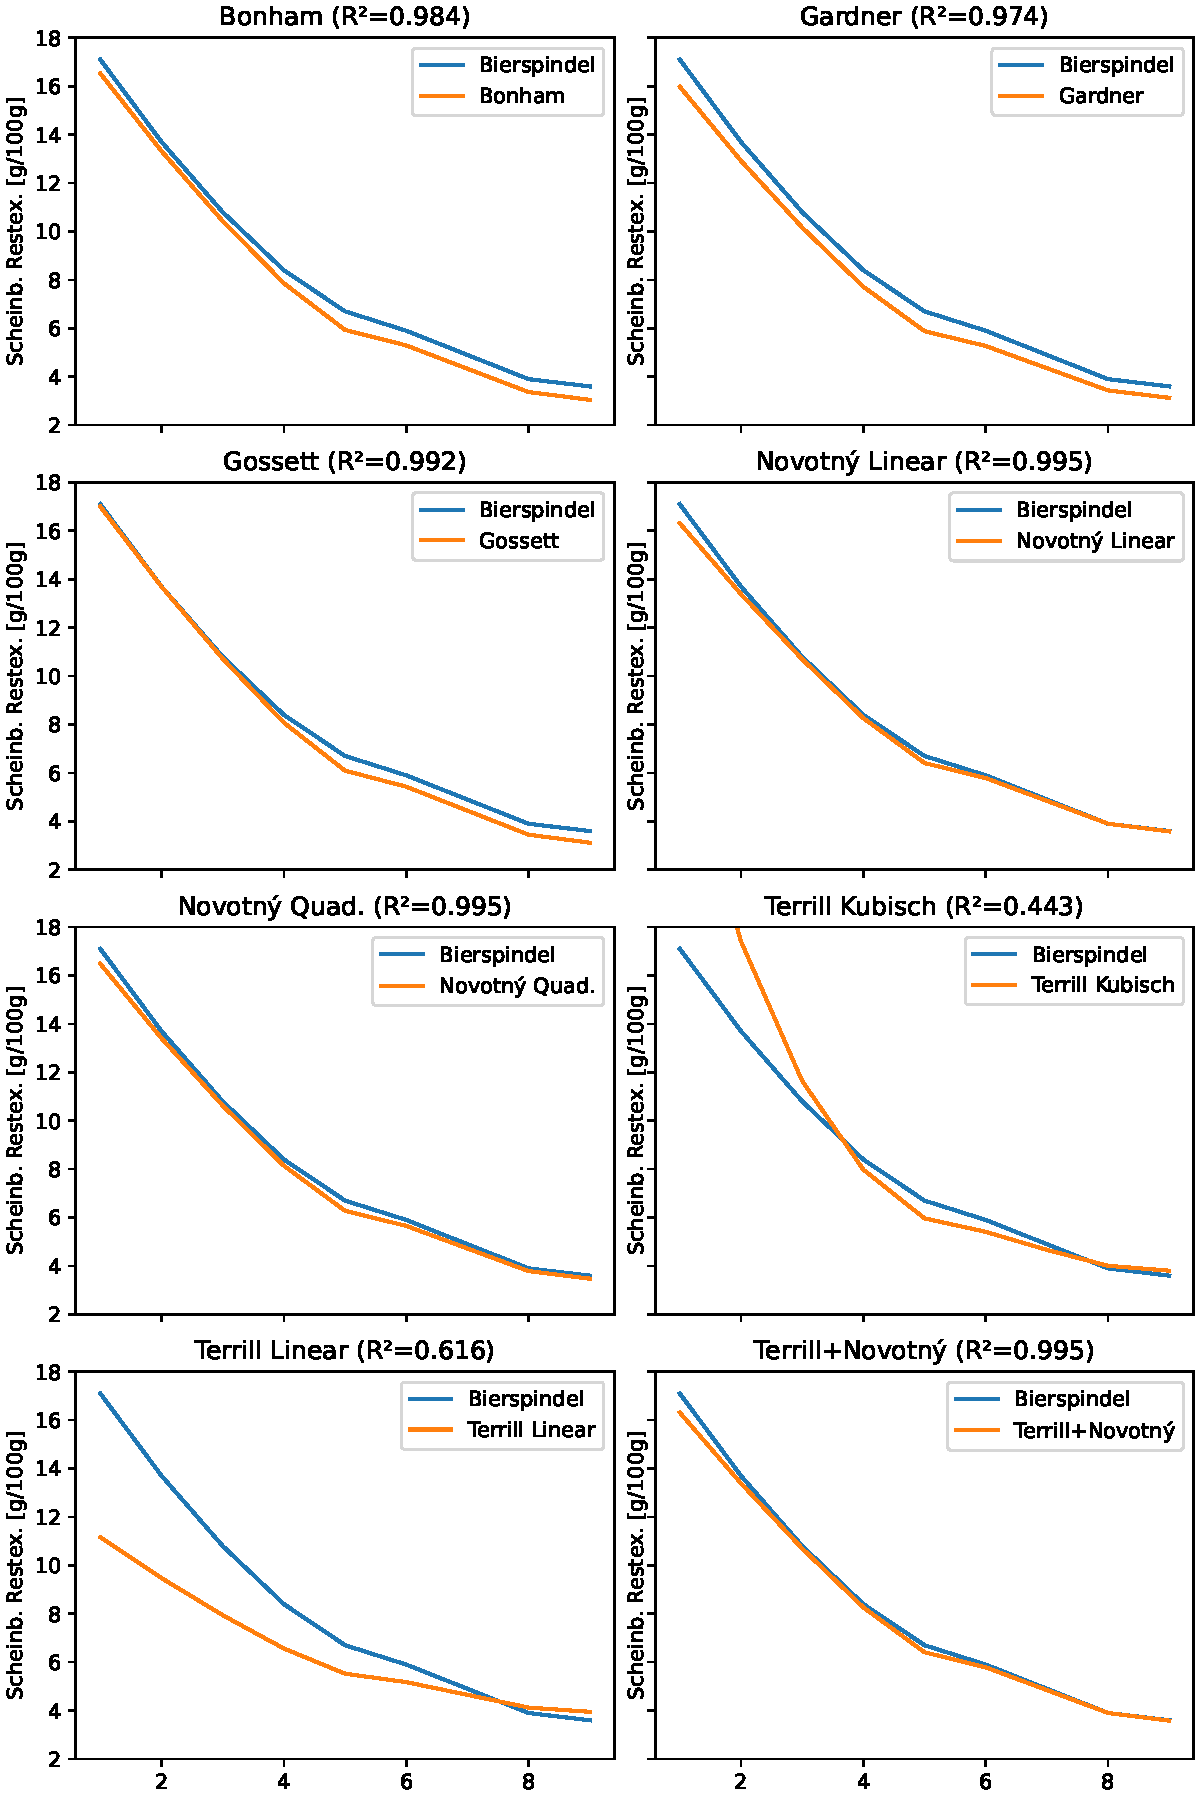
\includegraphics[width=14cm]{graph_fermentation.pdf}
\caption{Scheinbarer Restextrakt bei Gärverlauf (Ascher, 2021)}
\label{fig:novotnygraph}
\end{figure}

\begin{figure}[H]
\centering
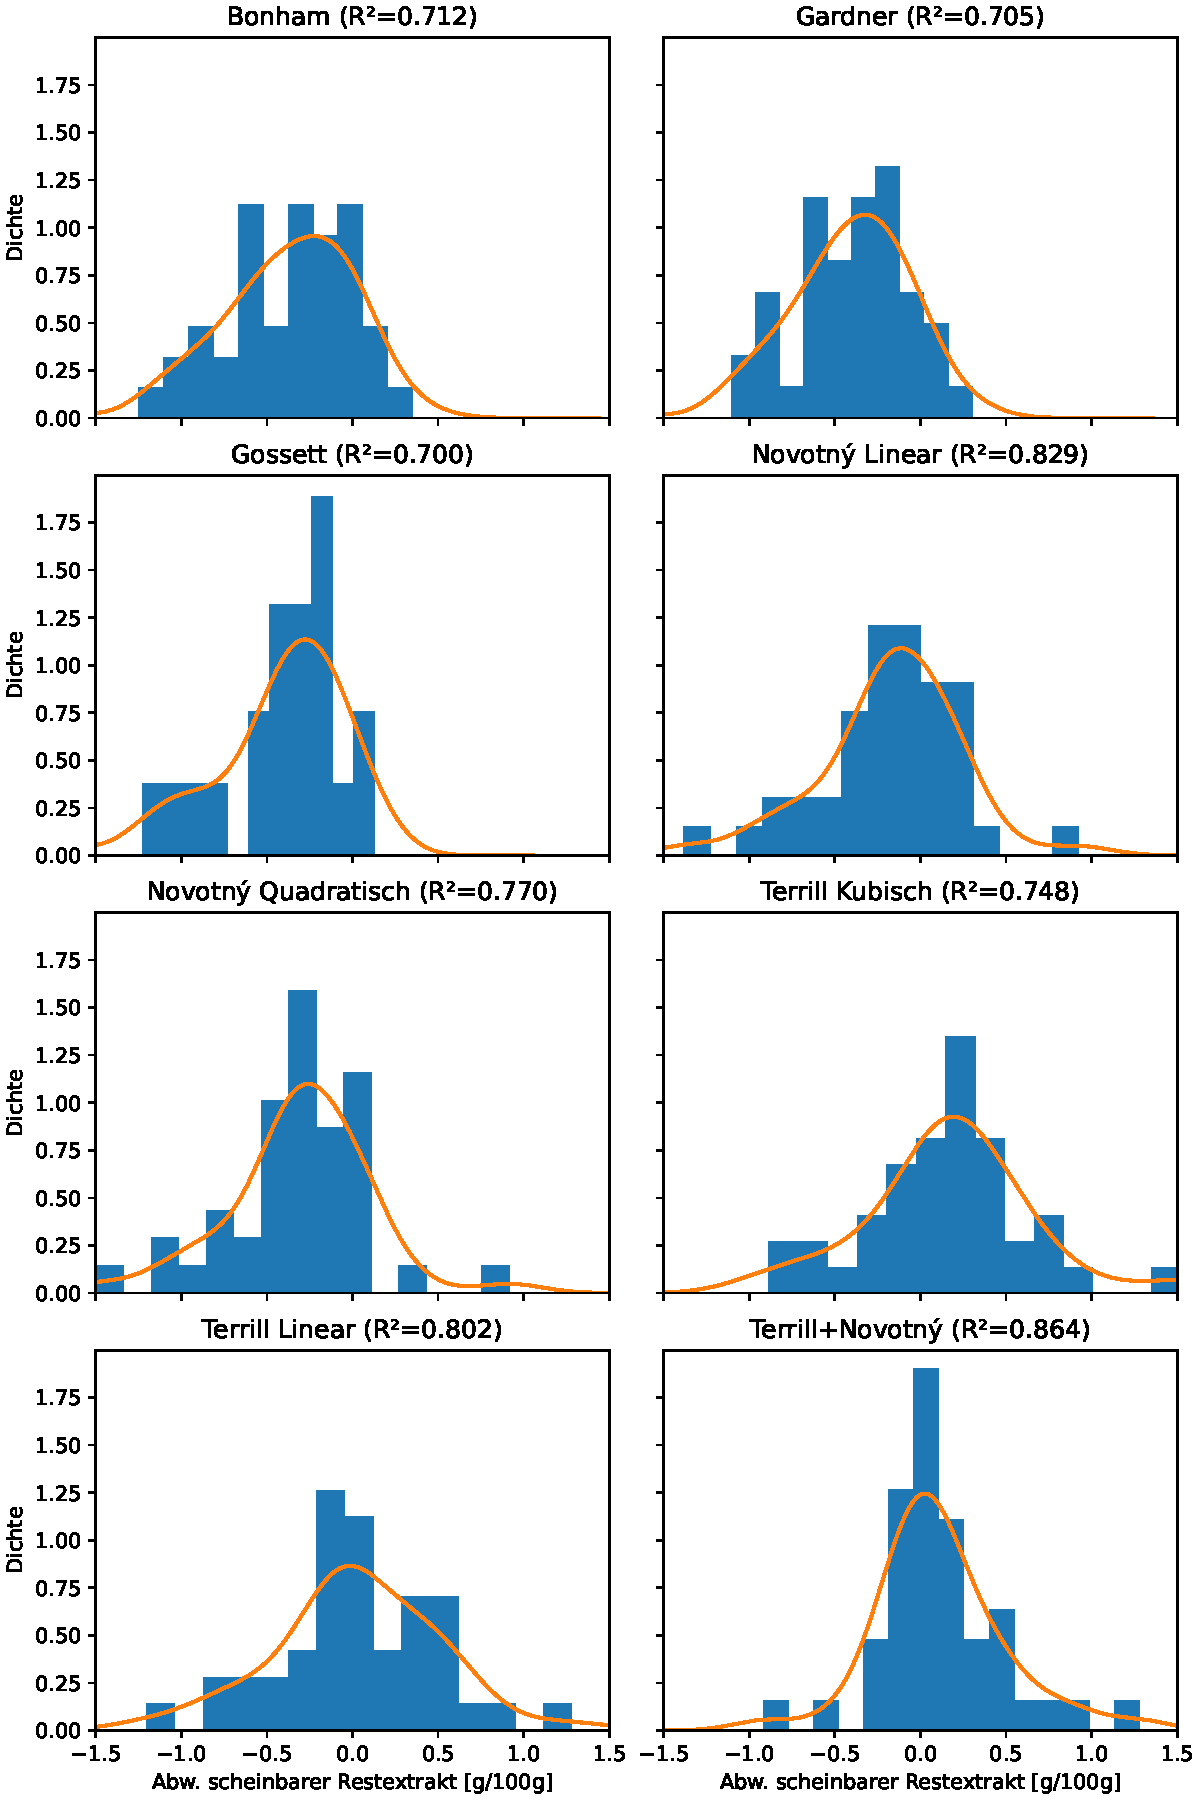
\includegraphics[width=14cm]{graph_ae.pdf}
\caption{Histogramme der Abweichungen des scheinbaren Restextrakts bei endvergorener Probe (Ascher, 2021)}
\label{fig:aegraph}
\end{figure}

\begin{table}[H]
\centering
\begin{tabular}{lrrrrrrrr}
\toprule
                     Statistik &    BO &   GA &    GO &    NL &    NQ &   TK &   TL &    TN \\
\midrule
        Endabweichung [g/100g] &  -0,6 & -0,5 &  -0,5 &  -0,0 &  -0,1 &  0,2 &  0,3 &  -0,0 \\
      Max. Abweichung [g/100g] &  -0,8 & -1,1 &  -0,6 &  -0,8 &  -0,6 &  9,0 & -5,9 &  -0,8 \\
  Mittlere Abweichung [g/100g] &  -0,5 & -0,7 &  -0,3 &  -0,2 &  -0,3 &  1,3 & -1,8 &  -0,2 \\
  Standardabweichung [g/100g]  &   0,1 &  0,2 &   0,2 &   0,2 &   0,2 &  3,2 &  2,1 &   0,2 \\
Abweichungen < 0,25 g/100g [\%] &   0,0 &  0,0 &  33,3 &  66,7 &  55,6 & 33,3 & 22,2 &  66,7 \\
Abweichungen < 0,50 g/100g [\%] &  22,2 & 22,2 &  88,9 &  88,9 &  88,9 & 55,6 & 33,3 &  88,9 \\
Abweichungen < 1,00 g/100g [\%] & 100,0 & 88,9 & 100,0 & 100,0 & 100,0 & 77,8 & 44,4 & 100,0 \\
\bottomrule
\end{tabular}
 \\
\vspace{2mm}
\small{BO=Bonham, GA=Gardner, GO=Gossett, NL=Novotný Lin., NQ=Novotný Quad., TK=Terrill Kub., TL=Terrill Lin.}
\caption{Abweichungen des scheinbaren Restextrakts bei Gärverlauf (Ascher, 2021)} 
\label{table:novotnytable}
\end{table}

\begin{table}[H]
\centering
\begin{tabular}{lrrrrrr}
\toprule
    Korrelation &  Max. Abw. [g/100g] &  Mittlere Abw. &  Standardabw. &  < 0,25 [\%] &  < 0,5 &  < 1,0 \\
\midrule
         Bonham &              -4,286 &         -0,372 &         0,690 &      40,000 & 62,500 & 86,250 \\
        Gardner &              -4,220 &         -0,406 &         0,643 &      37,500 & 67,500 & 90,000 \\
        Gossett &              -5,098 &         -1,043 &         0,857 &      13,750 & 20,000 & 58,750 \\
 Novotný Linear &              -4,270 &         -0,355 &         0,675 &      45,000 & 67,500 & 85,000 \\
  Novotný Quad. &              -4,287 &         -0,480 &         0,659 &      35,000 & 66,250 & 82,500 \\
Terrill Kubisch &              -1,988 &          0,044 &         0,726 &      35,000 & 48,750 & 81,250 \\
 Terrill Linear &              -1,966 &         -0,090 &         0,665 &      35,000 & 57,500 & 86,250 \\
Terrill+Novotný &              -1,966 &          0,024 &         0,578 &      48,750 & 71,250 & 87,500 \\
\bottomrule
\end{tabular}
 \\
\vspace{2mm}
\small{BO=Bonham, GA=Gardner, GO=Gossett, NL=Novotný Lin., NQ=Novotný Quad., TK=Terrill Kub., TL=Terrill Lin.}
\caption{Abweichungen des scheinbaren Restextrakts bei endvergorener Probe  (Ascher, 2021)}
\label{table:aetable}
\end{table}

\section*{Bestimmung des Alkoholgehalts und weiterer Kennzahlen}

Der durch die Balling Formel formulierte Zusammenhang zwischen
scheinbarem Restextrakt, wirklichem Restextrakt, Stammwürze
und Alkoholgehalt kann dazu verwendete werden, um aus der
Menge des während einer Gärung durch die Hefe konsumierten
Extrakts den daraus resultierenden Alkoholgehalt ohne aufwendigere
analytischer Verfahren als Näherungswert zu berechnen. Dafür muss
eine Messung der Stammwürze vor der Gärung und eine Messung des
scheinbaren Restextrakts während oder nach der Gärung durchgeführt
werden. \parencites[139\psq]{MEBAK2013}[137\psqq]{Spedding2016}

Bei Messungen mit einem Refraktometer ist dabei die
gemessene Stammwürze durch den Würze-Korrekturfaktor und
der gemessene scheinbare Restextrakt durch eine Korrelationsfunktion
zu korrigieren. Für die weitere Berechnung muss zuerst
der wirkliche Restextrakt als Näherungswert bestimmt werden.
Dies erfolgt anhand von \autoref{eq:calcre} auf Basis
der mit \autoref{eq:applywcf} ermittelten Stammwürze und
je nach Korrelationsmodell mit \autoref{eq:calcsgtop}
ermitteltem scheinbaren Restextrakt.

\begin{equation}
\rex\:[g/100g] = 0,1948 \cdot \oex + 0,8052 \cdot \aex
\label{eq:calcre} 
\end{equation}

Durch einsetzten der Stammwürze und des wirklichen Restextrakts
in \autoref{eq:calcabw} wird dann der Alkoholgehalt als
Gewichtsanteil berechnet. Um den Volumensanteil zu erhalten, ist
neben dem berechneten Ergebnis die durch die gewählte
Korrellationfunktion ermittelte spezifische Dichte
in \autoref{eq:calcabv} einzusetzen.

\begin{equation}
\abw\:[\%\:w/w] = \frac{\oex - \rex}{2,0665 - 1.0665 \cdot \oex / 100}
\label{eq:calcabw}
\end{equation}

\begin{equation}
\abv\:[\%\:v/v] = \frac{\abw \cdot \sg}{0,7907}
\label{eq:calcabv}
\end{equation}

Eine weitere Kennzahl, die aus den durchgeführten Messungen berechnet
werden kann, ist der Vergärungsgrad. Dieser gibt an, zu welchem
Anteil der ursprüngliche Extrakt während der Gärung konsumiert wurde.
Für den scheinbaren Restextrakt wird der scheinbare Vergärungsgrad
(Apparent Degree of Fermentation, \adftext) gemäß \autoref{eq:calcadf}
ermittelt. Der wirkliche Vergärdungsgrad (Real Degree of Fermentation,
\rdftext) ist nach Methode der American Society of Brewing Chemists
(ASBC) durch \autoref{eq:calcrdf} zu berechnen. Alternativ kann als
Näherung der scheinbare Vergärungsgrad mit dem Ballingschen
Umrechnungsaktor 0,81 multipliziert werden.
\parencites[131,137\psq]{MEBAK2013}[116,125]{Spedding2016}{Speers2015}

\begin{equation}
\adf\:[\%]= 100 \cdot \frac{\oex - \aex}{\oex}
\label{eq:calcadf}
\end{equation}

\begin{equation}
\rdf\:[\%] = 100 \cdot \frac{\oex - \rex}{\oex} \cdot \frac{1}{1 - 0,005161 \cdot \rex}
\label{eq:calcrdf}
\end{equation}

Die auf den Etiketten von Bierflaschen abgedruckten Nährwertangaben sind
zwar nur in Verbindung mit chemisch analytischen Verfahren feststellbar,
lassen sich aber mithilfe von \autoref{eq:calckj} und \autoref{eq:calckcal}
für eine Schnellanalyse abschätzen \parencite[161]{MEBAK2013}. 

\begin{equation}
kJ/100ml = \sg \cdot (14 \cdot \rex + 29 \cdot \abw)
\label{eq:calckj}
\end{equation}

\begin{equation}
kcal/100ml = \sg \cdot (3,5 \cdot \rex + 7 \cdot \abw)
\label{eq:calckcal}
\end{equation}

Eine Implementierung aller vorgestellten Berechnungen in der Form eines
Refraktometer-Rechners ist über \url{https://aschet.github.io/refractometer/}
abrufbar.

\section*{Berechnungsbespiel}

Bei einer mit einem Refraktometer gemessene Stammwürze von $\bxi = 12$
und einem Restextrakt von $\bxf = 6$ ist bei einem Würze-Korrekturfaktor
von $\wcf = 1,04$ mithilfe der linearen Terrill Formel
(\autoref{eq:terrilllinear}) der Alkoholgehalt des gemessenen Bieres
zu berechnen. Unter Anwendung von \autoref{eq:applywcf},
\autoref{eq:terrilllinear}, \autoref{eq:calcsgtop},
\autoref{eq:calcre}, \autoref{eq:calcabw} und \autoref{eq:calcabv} ergibt
sich folgender Berechnungsweg:

\begin{align*}
\bxic\:[\degree P] &= 12 / 1,04 = 11,54 \\
\bxfc\:[g/100g] &= 6 / 1,04 = 5,77 \\
\sg\:[g/ml] &= 1 - 0,00085683 \cdot 11,54 + 0,0034941 \cdot 5,77 = 1,010 \\
\aex\:[g/100g] &= -205,347 \cdot 1,010^2 + 668,72 \cdot 1,010 - 463,37 = 2,63 \\
\rex\:[g/100g] &= 0,1948 \cdot 11,54 + 0,8052 \cdot 2,63 = 4,37 \\
\abw\:[\%\:w/w] &= \frac{11,54 - 4,37}{2,0665 - 1,0665 \cdot 11,54 / 100} = 3,69 \\
\abv\:[\%\:v/v] &= \frac{3,69 \cdot 1,010}{0,7907} = 4,71
\end{align*}

\section*{Zusammenfassung}

Die relevanten Eckpunkte dieses Artikels sind:

\begin{itemize}
\item Refraktometer messen auf Basis der Brechung des Lichts. Im
Heimbrauumfeld eingesetzte Handgeräte sind zumeist mit einer 
Brix-Skala ausgestattet.
\item Mit einem Refraktometer erfasste Messwerte müssen umgerechnet
werden. Bei Messungen vor einer Gärung (Stammwürze) ist der
Würze-Korrekturfaktor anzuwenden. Messungen nach
einer Gärung unterliegen einer Verfälschung aufgrund des gebildeten
Alkohols. Zur Korrektur wird ein Messwert mithilfe einer
Korrelationsfunktion transformiert.
\item Vor einer Messung sollte eine Kalibrierung und Justierung
mit destilliertem Wasser bei Raumtemperatur erfolgen.
\item Proben sind für die Messung aufzubereiten. Heiße Würze
sollte in einem abgedeckten Container auf Raumtemperatur
abgekühlt werden. Während oder nach einer Gärung entnommene
Proben müssen bei der Messung frei von Schwebstoffen und Gasen sein.
Enthaltenes \ch{CO2} lässt sich durch wiederholtes Schütteln
entfernen. Enthaltene Hefe sedimentiert nach längerer Wartezeit.
\item Zur Bestimmung des Alkoholgehalts ist eine Messung
vor und eine nach einer Gärung durchzuführen. Mithilfe eines
Refraktometer-Rechners lässt sich dann der Alkoholgehalt
als Näherungswert berechnen: \url{https://aschet.github.io/refractometer/}

\end{itemize}

\printbibliography[title=Quellen]

\end{document}